\documentclass[../03-Architecture.tex]{subfiles}
\begin{document}

\section{Computer Graphics in Web-Environments}
\label{sec:cg-web}
% ************************************************

In this section we give a brief overview of graphics programming
fundamentals in general and in web-environments. These fundamentals
are the concepts of {\threedmodel} data representation in
Section~\ref{sub:model-representation} and render loops and scene
graphs in Section~\ref{sub:render-and-graph}.

\subsection{{\threedmodel} Representation}
\label{sub:model-representation}

This section explains which data structures and disk-formats are used
to represent {\threedmodel}s. First, we explain the terminology of
meshes. Secondly, we look at the {\stlfile} format.

The model geometry is represented by a set of connected polygons,
approximating the model surface. These connected polygons form a mesh.
Figure~\ref{fig:term-mesh:mesh} shows a mesh. We use triangles as
polygons, because then we benefit from hardware acceleration. A
triangle in the mesh is called face. Each face is described by a list
of three points in 3D-space. Such a point is called vertex. A single
vertex is described by three floating point numbers for the x-, y- and
z-coordinates. An edge is the line between two connected vertices
\cite[p.~3]{cg-intro}. Figure~\ref{fig:term-mesh:face} illustrates the
terminology.

\begin{figure}[h]
  \centering
  \begin{subfigure}[b]{0.49\textwidth}
    \centering
    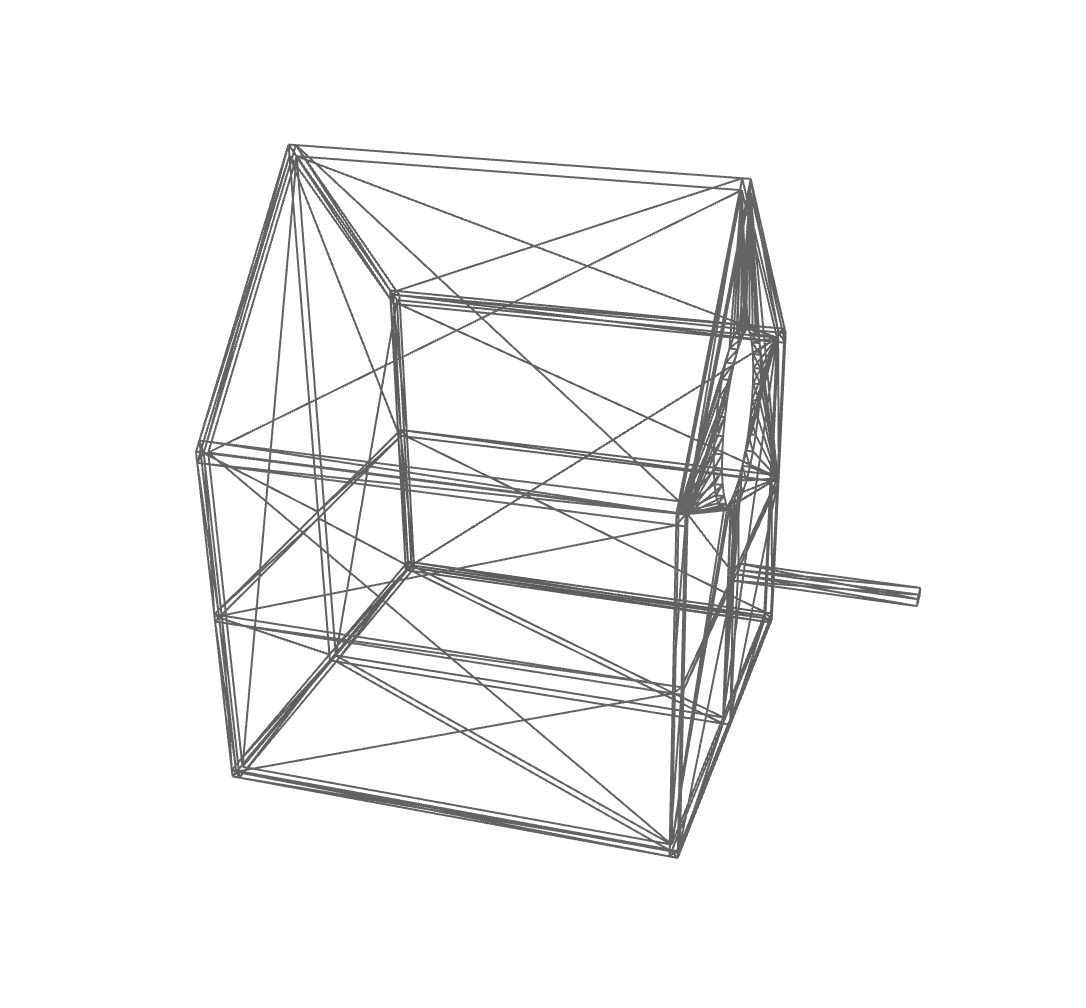
\includegraphics[width=\textwidth]{03-architecture-birdhouse}
    \caption{A triangle mesh of a bird house.}
    \label{fig:term-mesh:mesh}
  \end{subfigure}
  \begin{subfigure}[b]{0.49\textwidth}
    \centering
    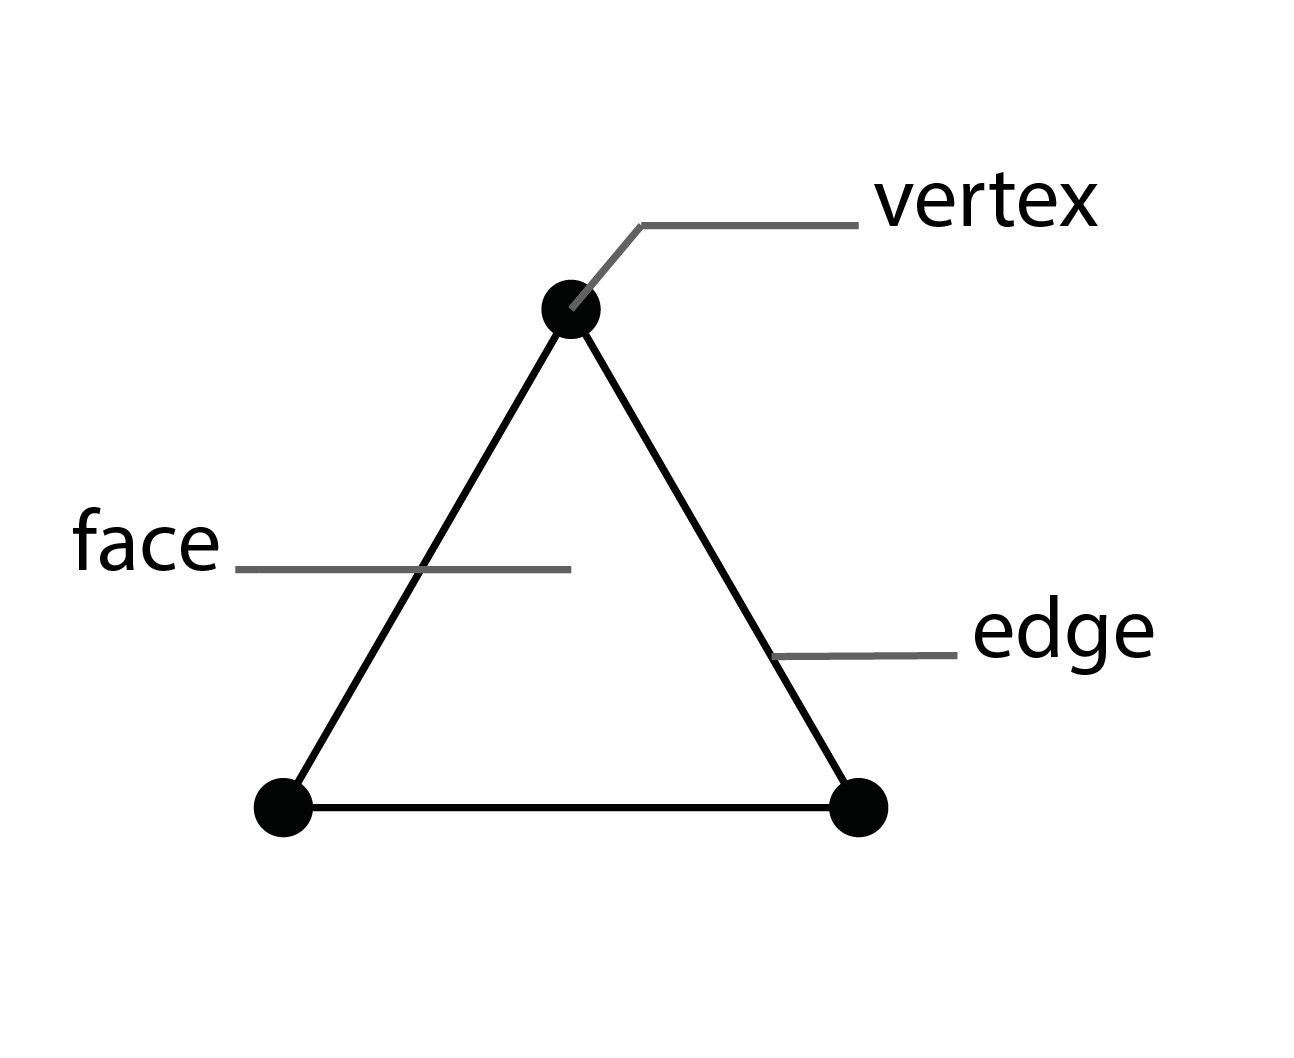
\includegraphics[width=\textwidth]{03-architecture-mesh-terminology}
    \caption{A single face with vertices and edges.}
    \label{fig:term-mesh:face}
  \end{subfigure}
  \caption{Terminology of a Mesh}
  \label{fig:term-mesh}
\end{figure}

We only support geometry which is arranged in two-manifold meshes.
Two-manifoldness is a constraint on the mesh, which requires each egde
to exactly touch two neighboring faces. Figure~\ref{fig:non-manifold}
shows a comparison of a manifold and non-manifold part of a mesh. It
follows then, that each triangular face has to have three adjacent
faces. Thus, the constraint enforces the mesh to be a fully connected
graph without holes \cite[p.~28]{master-thesis}. We require
two-manifoldness to make
sophisticated assumption when designing the conversion algorithms.

\note{make own figure for non-manifold mesh}

\begin{figure}[h]
  \centering
  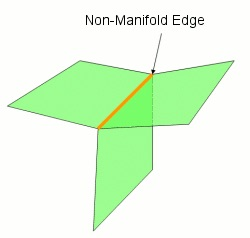
\includegraphics[width=0.6\textwidth]{03-architecture-non-manifold}
  \caption{A non-manifold cutout of a mesh.}
  \label{fig:non-manifold}
\end{figure}

The Standard Tessellation Language (STL) format is a common file
format for {\threedmodel} representation in the context of
{\threedprinting}. We support the {\stlfile} format, because our goal
is to make models, built for a {\threedprinter}, available for the
{\lasercutter}. An {\stlfile} consists of a list of faces associated
with their face normal. Each face is given as a list of vertices. We
cannot say in which direction the face points judging only from the
vertices. The face normal determines the orientation of the face.
Listing~\ref{alg:stl-file} shows an {\stlfile} in ASCII encoding. For
saving disk-space, the file is mostly stored in a binary format
\cite[p.~8]{stl-file}.

\begin{listing}
\centering
\begin{CVerbatim}
solid name
 facet normal n1 n2 n3
  outer loop
   vertex p1x p1y p1z
   vertex p2x p2y p2z
   vertex p3x p3y p3z
  endloop
 endfacet
endsolid name
\end{CVerbatim}
\caption{General format of a STL-file in ASCII encoding.}
\label{alg:stl-file}
\end{listing}

Reconstructing the original {\threedmodel} from an {\stlfile} does not
always result in an one-to-one solution. The vertices are stored with
floating point numbers instead of referring to the same vertex with an
index. Thus, we have to assume, that two overlapping points represent
an identical vertex. We use the library {\meshlib} to create an
indexed face-vertex-mesh from the possibly ambiguous {\stlfile}. With
{\meshlib}, we can convert the face-vertex-mesh representation to a
{\threejs} geometry. With a {\threejs} geometry, we can render a
{\threedmodel} in {\convertify}.

To support a variety of {\threedprinter} optimized models, we use the
{\stlfile} format. We import the files with the {\meshlib} library.
The imported face-vertex-mesh structure is then converted for usage
with {\threejs}. The section below explains how the {\threejs}
representation is displayed on the screen.

\subsection{Render Loop and Scene Graphs}
\label{sub:render-and-graph}

To understand how {\convertify} and {\platener} work, we have to
familiarize with the concepts of rendering and scene graphs first.

A typical pattern in graphics software is the render loop.
Rendering is the process of turning the {\threedmodel}
representation into an array of pixels which can be
displayed on the screen~\cite[p.~2]{intro-cg}. We have to
render the {\threedmodel} in a continuous loop, because we
do not want to produce a single static image. The render
loop pattern consists of three steps: processing input,
updating the {\threedmodel} representation and
rendering~\cite{gamedev-gameloop}.
Figure~\ref{fig:render-loop} shows an exemplary flow.

\begin{figure}[h]
  \centering
  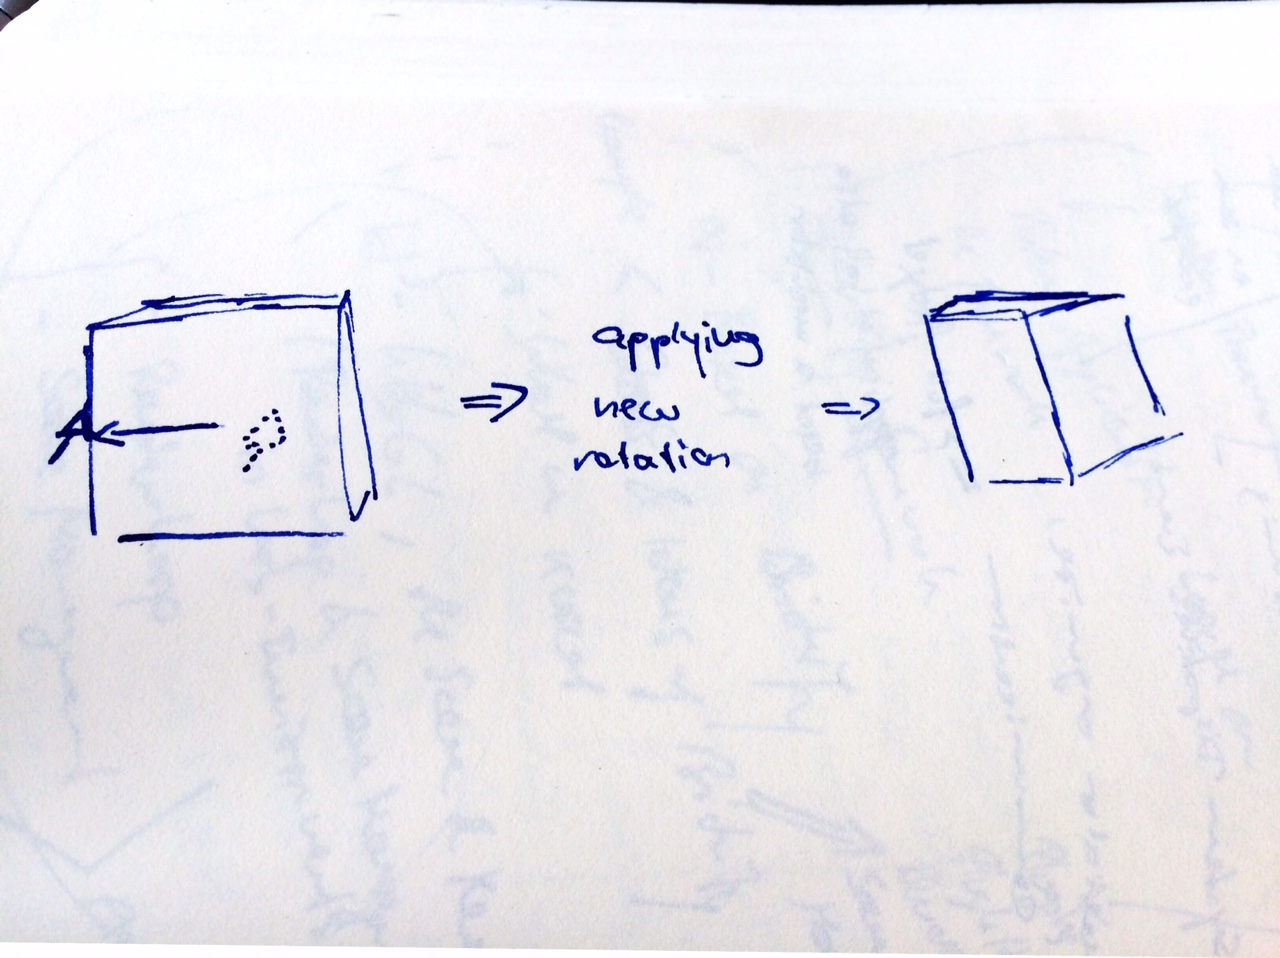
\includegraphics[width=1\columnwidth]{03-architecture-render-loop}
  \caption{Touch input is processed by the render loop.}
  \label{fig:render-loop}
\end{figure}

Each object is part of a scene. A scene is the visual space, in which
the rendered objects can be seen. We use representations of objects
which are organized in a hierarchical tree data structure. We refer to
this hierarchical structure as scene graph\ref{}\myNotes{reference
  scene graph data structure}. A simple scene graph is depicted in
Figure~\ref{}. The shown graph contains a box as single root node. The
sides of the box are children of the root node. With this abstraction
we can easily apply transformations to parts of the model only,
without necessarily touching each face or vertex. Every object that
is recognized by {\convertify}, is part of a scene graph. Finally, the
vertices of an object in the scene graph are rendered to the screen.

\begin{figure}[H]
  \centering
  \begin{subfigure}[b]{0.49\textwidth}
    \centering
    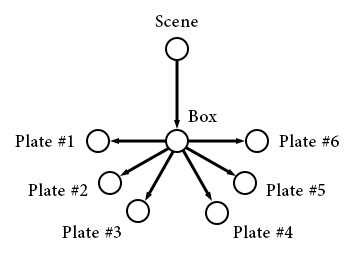
\includegraphics[width=\textwidth]{03-architecture-scene-graph-abstract}
    \caption{Graph notation of the composed box.}
    \label{fig:scene-graph:abstract}
  \end{subfigure}
  \begin{subfigure}[b]{0.49\textwidth}
    \centering
    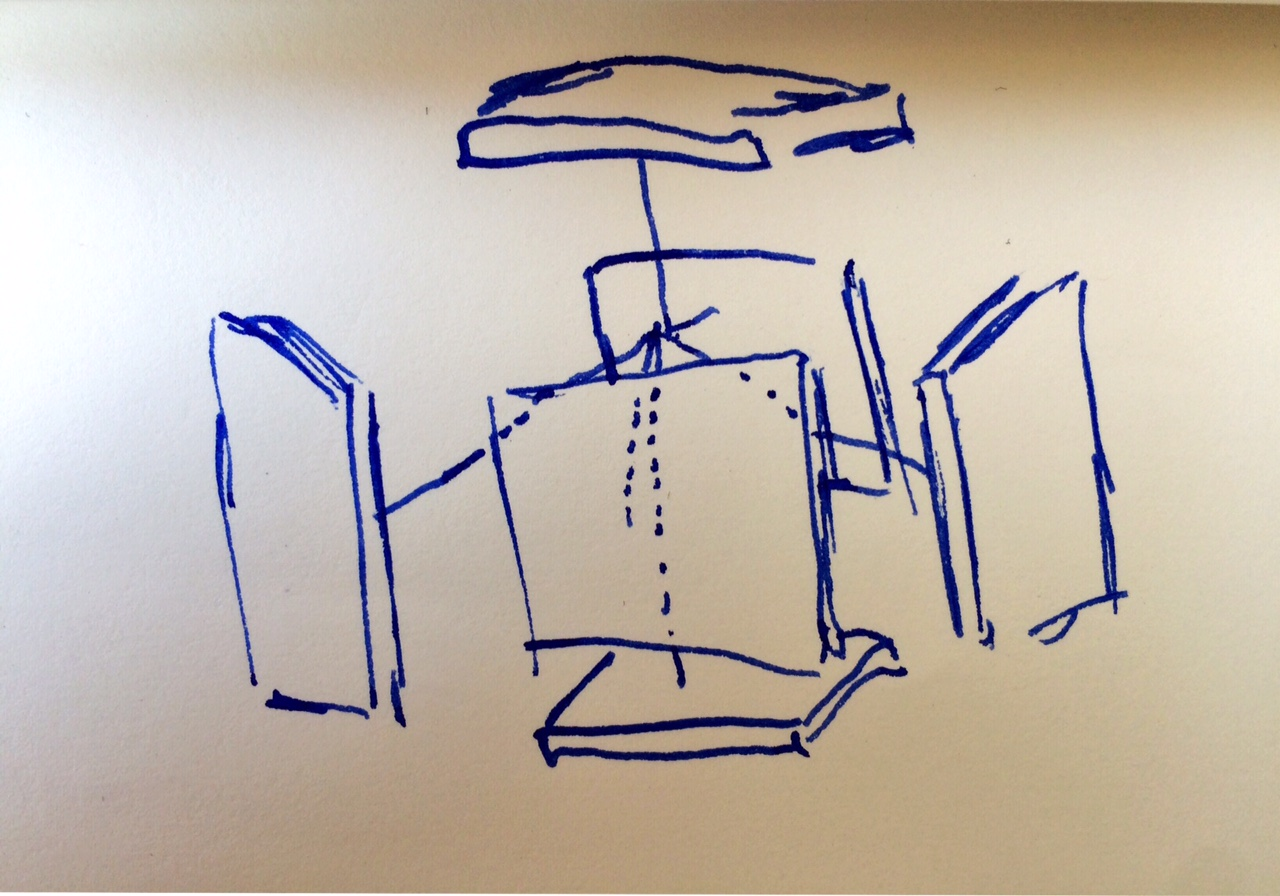
\includegraphics[width=1\textwidth]{03-architecture-scene-graph-visual}
    \caption{Rendered box in an explosion view, showing decomposition into plates.}
    \label{fig:scene-graph:visual}
  \end{subfigure}
  \caption{A scene graph showing a box, composed of plates.}
  \label{fig:scene-graph}
\end{figure}


The framework {\convertify} uses common computer graphics
patterns like render loops and scene graphs. With the help
of WebGL and {\threejs} we are able to bring these concepts
into a web-environment.

\end{document}

%%% Local Variables:
%%% mode: latex
%%% TeX-master: "../03-Architecture"
%%% TeX-command-extra-options: "-shell-escape"
%%% End:
